\section{Problem 2: propagation, fidelity and effective range}\label{sec:q2}

\subsection{From three correlations to one fidelity index}

For each call type the archive supplies three correlation series measured against the 1 m
reference recording: a spectrogram correlation, an amplitude-spectrum correlation and an
envelope correlation, each at seven distances from 4 to 256 m. The problem requires all three to
enter the analysis jointly, so we define
\begin{equation}\label{eq:fidelity}
  F_t(d) \;=\; \sum_{m\in\{\mathrm{spec},\mathrm{amp},\mathrm{env}\}} w_m\, r_{m,t}(d),
  \qquad \sum_m w_m = 1 ,
\end{equation}
with equal weights as the baseline. The index lies in $[0,1]$ by construction, since each $r$ is
a correlation, and requires no separate normalisation: at 4 m all three call types already sit
between 0.63 and 0.92, so the scale is anchored by the data rather than by an arbitrary constant.

The three components are not independent evidence. The spectrogram and amplitude-spectrum
correlations are highly correlated across call types (per-type correlations of 0.81--0.97),
although at the level of individual trials the agreement is weaker and varies with distance
(from 0.56 at short range to 0.99). A principal-component analysis of
the three gives a first component explaining 73.5--85.2\% of the variance with loadings of about
0.35, 0.35 and 0.30. Equal weighting therefore places two thirds of the weight on what is
effectively one dimension. We keep equal weights as the baseline because it is the least
assumption-laden choice, report the principal-component weights as an alternative, and treat the
envelope weight as the sensitivity parameter that matters most
(Section~\ref{sec:q2-sens}).

Table~\ref{tab:q2-raw} gives the raw means that enter Equation~\eqref{eq:fidelity}, and
Figure~\ref{fig:q2-fidelity} shows the resulting curves.

\begin{table}[htbp]
  \centering
  \caption{Mean correlation with the 1 m reference recording, by distance, call type and metric
  (s = spectrogram, a = amplitude spectrum, e = envelope). Each value is a mean over the available
  trials of that distance; $n$ varies from 190 to 300.}\label{tab:q2-raw}
  \scriptsize
  \setlength{\tabcolsep}{3.4pt}
  \begin{tabular}{lrrrrrrrrr}
    \toprule
    & \multicolumn{3}{c}{flat} & \multicolumn{3}{c}{mod} & \multicolumn{3}{c}{tv} \\
    \cmidrule(lr){2-4}\cmidrule(lr){5-7}\cmidrule(lr){8-10}
    Distance (m) & s & a & e & s & a & e & s & a & e \\
    \midrule
    4 & 0.908 & 0.923 & 0.650 & 0.872 & 0.876 & 0.675 & 0.824 & 0.825 & 0.626 \\
    8 & 0.892 & 0.868 & 0.595 & 0.913 & 0.918 & 0.754 & 0.880 & 0.880 & 0.634 \\
    16 & 0.905 & 0.918 & 0.657 & 0.841 & 0.844 & 0.656 & 0.789 & 0.790 & 0.515 \\
    32 & 0.869 & 0.755 & 0.529 & 0.834 & 0.847 & 0.560 & 0.811 & 0.819 & 0.506 \\
    64 & 0.733 & 0.712 & 0.343 & 0.842 & 0.860 & 0.599 & 0.846 & 0.849 & 0.562 \\
    128 & 0.412 & 0.453 & 0.211 & 0.618 & 0.680 & 0.362 & 0.740 & 0.772 & 0.449 \\
    256 & 0.166 & 0.192 & 0.170 & 0.250 & 0.278 & 0.223 & 0.318 & 0.371 & 0.139 \\
    \bottomrule
  \end{tabular}
\end{table}


\begin{figure}[htbp]
  \centering
  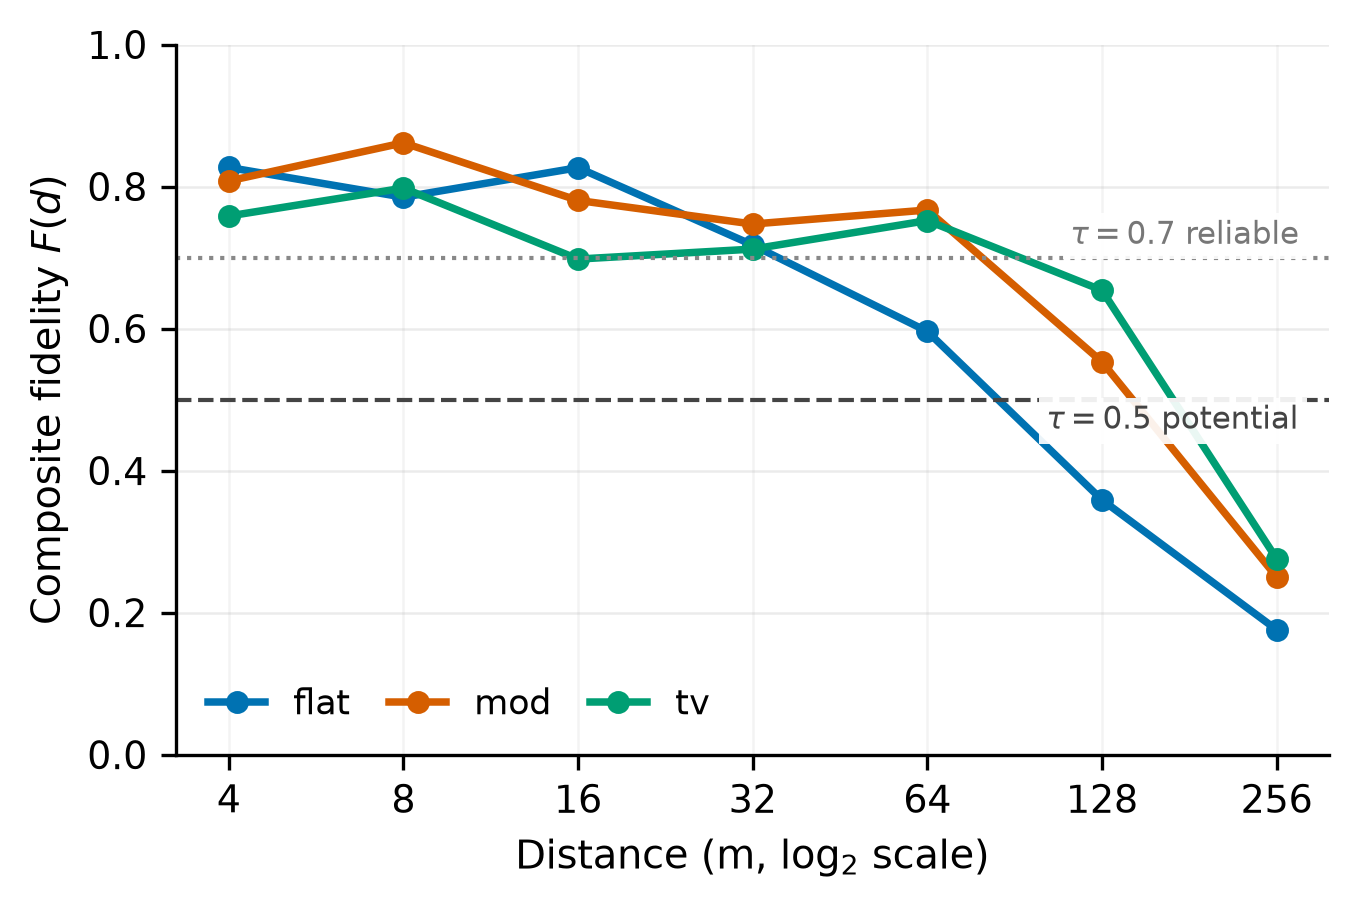
\includegraphics[width=0.44\textwidth]{figs/fig2_fidelity.png}
  \caption{Composite fidelity against distance with the two operational thresholds. The curves
  are not monotone at short range: modulated and two-voice fidelity rise from 4 to 8 m.}\label{fig:q2-fidelity}
\end{figure}

Three patterns are visible before any model is fitted. Fidelity is nearly flat to 32 m for all
three types. It collapses between 64 and 256 m, with the two-voice call retaining the most at
128 m (0.654 against 0.553 for modulated and 0.359 for flat). And the envelope correlation starts
far below the other two (0.65 at 4 m) and contributes the steepest decline, which is why it
behaves as the strictest of the three filters.

\subsection{Three performance models and a threshold scheme}

The problem asks for a separate degradation model for each call type. We fit three families to
the seven distance means, because with seven points the shape of the curve is not identified by
the data alone.

\begin{itemize}[leftmargin=1.5em,itemsep=2pt]
  \item A \textbf{monotone interpolation} on the $\log_2$ distance axis, which imposes only that
        fidelity does not increase with distance. This is the primary curve and the one used for
        the radii reported below.
  \item A \textbf{generalised additive model} $F_t(d)=\beta_0+s_t(d)+\varepsilon$ with a penalised
        spline, mirroring the official analysis code. The effective degrees of freedom are 2.93
        (flat), 2.00 (mod) and 2.88 (tv); the value of exactly 2.00 for modulated means the
        smoother has collapsed to a linear trend, not that the true relation is linear.
  \item Two \textbf{Weibull-type decays}, four-parameter
        $F=b+(a-b)\exp[-(d/\lambda)^k]$ and three-parameter ($b=0$), fitted by constrained
        nonlinear least squares.
\end{itemize}

The threshold scheme converts fidelity into a graded claim about recognisability.
Table~\ref{tab:q2-thresholds} states the three tiers. They are operational definitions chosen to
span the range a receiver might use; the data cannot locate a perceptual boundary, and we do not
claim that they do.

\begin{table}[htbp]
  \centering
  \caption{Three-tier recognition scheme. The two focal criteria are shown in bold.}\label{tab:q2-thresholds}
  \small
  \begin{tabular}{llll}
    \toprule
    Tier & $\tau$ & Reading & Role \\
    \midrule
    Potential recognition & \textbf{0.5} & the signal is still distinguishable from noise & \textbf{focal criterion 1} \\
    Intermediate & 0.6 & the pattern is recoverable with effort & reported for continuity \\
    Reliable recognition & \textbf{0.7} & the pattern is recoverable without effort & \textbf{focal criterion 2} \\
    \bottomrule
  \end{tabular}
\end{table}

\subsection{Effective communication range}

Inverting the monotone curve gives the effective range $d^*(\tau)=\{d: F_t(d)=\tau\}$, computed by
interpolation and reported with a bootstrap interval over the available records.
Table~\ref{tab:q2-ranges} gives the six focal radii together with the intermediate tier.

\begin{table}[htbp]
  \centering
  \caption{Effective range (m) by call type and criterion. Brackets: bootstrap interval over
  records; see the note on interval width in the text.}\label{tab:q2-ranges}
  \small
  \begin{tabular}{lrrr}
    \toprule
    Criterion & flat & mod & tv \\
    \midrule
    Potential, $\tau=0.5$ & 84.7 [83.1, 86.4] & 144.6 [140.6, 148.2] & 169.7 [168.6, 170.9] \\
    Intermediate, $\tau=0.6$ & 62.6 & 109.2 & 141.3 \\
    Reliable, $\tau=0.7$ & 35.4 [32.6, 37.9] & 77.7 [76.1, 79.5] & 79.2 [76.0, 82.5] \\
    \bottomrule
  \end{tabular}
\end{table}

These intervals resample individual records and assume exchangeability, which the data violate:
the 300 rows form 30 blocks of ten, so a block bootstrap would widen them by a factor of about
2.5. The brackets should be read as lower bounds; the model-family range below is the more
honest summary.

At the potential-recognition criterion the ordering is unambiguous: two-voice calls travel
roughly twice as far as flat calls, and the confidence intervals do not overlap. At the
reliable-recognition criterion the two-voice advantage disappears: 79.2 m against 77.7 m for
modulated, with overlapping intervals. This is not a contradiction but a change of question:
a strict criterion asks whether the fine structure survives, and by that standard the two-voice
call is no better than the modulated one.

The long-distance comparison makes the same point quantitatively. A trapezoidal average on the
log-distance axis over 64--256 m gives 0.576 (tv), 0.528 (mod) and 0.372 (flat). At 128 m the
values are 0.654, 0.553 and 0.359, and at 256 m 0.276, 0.250 and 0.176. Two-voice calls lead at
both of these distances, but modulated calls lead at 64 m (0.757 against 0.721), so the
two-voice advantage is a property of the far field rather than of the whole range; the margin
over modulated shrinks from 0.10 at 128 m to 0.03 at 256 m.

\subsection{Sensitivity: weights, thresholds and model family}\label{sec:q2-sens}

Three dimensions move the answer, and two of them move it more than the sampling error does.

\begin{table}[htbp]
  \centering
  \caption{Effective ranges (m) under four fusion weightings, at the two focal thresholds.}\label{tab:q2-sens}
  \small
  \begin{tabular}{llrrr}
    \toprule
    Threshold & Weighting & flat & mod & tv \\
    \midrule
    $\tau=0.5$ & equal & 84.7 & 144.6 & 169.7 \\
               & spectrogram 0.5 & 90.8 & 148.8 & 175.0 \\
               & amplitude spectrum 0.5 & 91.5 & 153.2 & 178.3 \\
               & envelope 0.5 & 71.3 & 129.8 & 155.9 \\
    \midrule
    $\tau=0.7$ & equal & 35.4 & 77.7 & 79.2 \\
               & spectrogram 0.5 & 43.5 & 82.8 & 99.9 \\
               & amplitude spectrum 0.5 & 38.4 & 85.2 & 106.2 \\
               & envelope 0.5 & 25.5 & 66.8 & \textbf{12.1} \\
    \bottomrule
  \end{tabular}
\end{table}

The envelope row at $\tau=0.7$ is the single most consequential number in Problem~2. Putting half
the weight on the envelope correlation cuts the two-voice radius from 79 m to 12 m and reverses
the ranking, because the two-voice envelope correlation at 256 m is the lowest of the three
(0.139 against 0.170 for flat and 0.223 for modulated), even though its spectrogram correlation
is the highest. The claim ``two-voice calls travel furthest'' is therefore true for the spectral
metrics, false for the envelope, and true of the equal-weight composite — a statement about
metric-dependence that we carry into Section~\ref{sec:q4}.

The third dimension is model family. Table~\ref{tab:q2-models} compares the three fitted
families by leave-one-distance-out RMSE.

\begin{table}[htbp]
  \centering
  \caption{Leave-one-distance-out RMSE by model family. Lower is better.}\label{tab:q2-models}
  \small
  \begin{tabular}{lrrr}
    \toprule
    Model & flat & mod & tv \\
    \midrule
    Distance GAM & 0.1232 & 0.0489 & 0.1215 \\
    Four-parameter Weibull & 0.0327 & 0.0603 & 0.1164 \\
    Three-parameter Weibull & 0.0457 & 0.0563 & 0.1163 \\
    \bottomrule
  \end{tabular}
\end{table}

Converting each fitted model into effective distances gives a different picture at each
tier. At $\tau=0.5$ the GAM returns 88.3, 151.8 and 182.1 m for flat, modulated and
two-voice; the three-parameter Weibull returns 89.7, 151.8 and 188.3 m; the four-parameter
Weibull returns 86.6, 146.0 and 144.9 m. At $\tau=0.7$ the corresponding values are 34.0,
64.3 and 89.2 m (GAM) and 35.9, 76.6 and 101.3 m (three-parameter Weibull).

The four-parameter Weibull puts modulated (146.0 m) marginally ahead of two-voice
(144.9 m), whereas the GAM, the three-parameter Weibull and the monotone interpolation all put
two-voice ahead. The four-parameter fit also drives its shape parameter to the imposed upper
bound ($k=10$) and its asymptotic value to the observed 256 m mean, which is a symptom of
over-parameterisation rather than evidence of a steep cliff. We therefore treat the Weibull
fits as model-family sensitivity, not as a replacement for the primary curve.

\subsection{Hand-off to Problem 4}

Problem~4 needs the fidelity surface on the same distance grid as the playback design. We pass on
$F_t(d)$ at 4, 8, 16, 32, 64, 128 and 256 m from the equal-weight composite, together with two
statements that constrain how it may be used: the values at 4--32 m are nearly flat and ordered
differently at different distances (flat leads at 16 m, modulated at 64 m), so no single ordering
holds at short range; and the two-voice advantage at long range is a property of the spectral
metrics, not of the envelope.
